\section{What is a Genetic Algorithm?}
\begin{figure}[h]
	\centering
		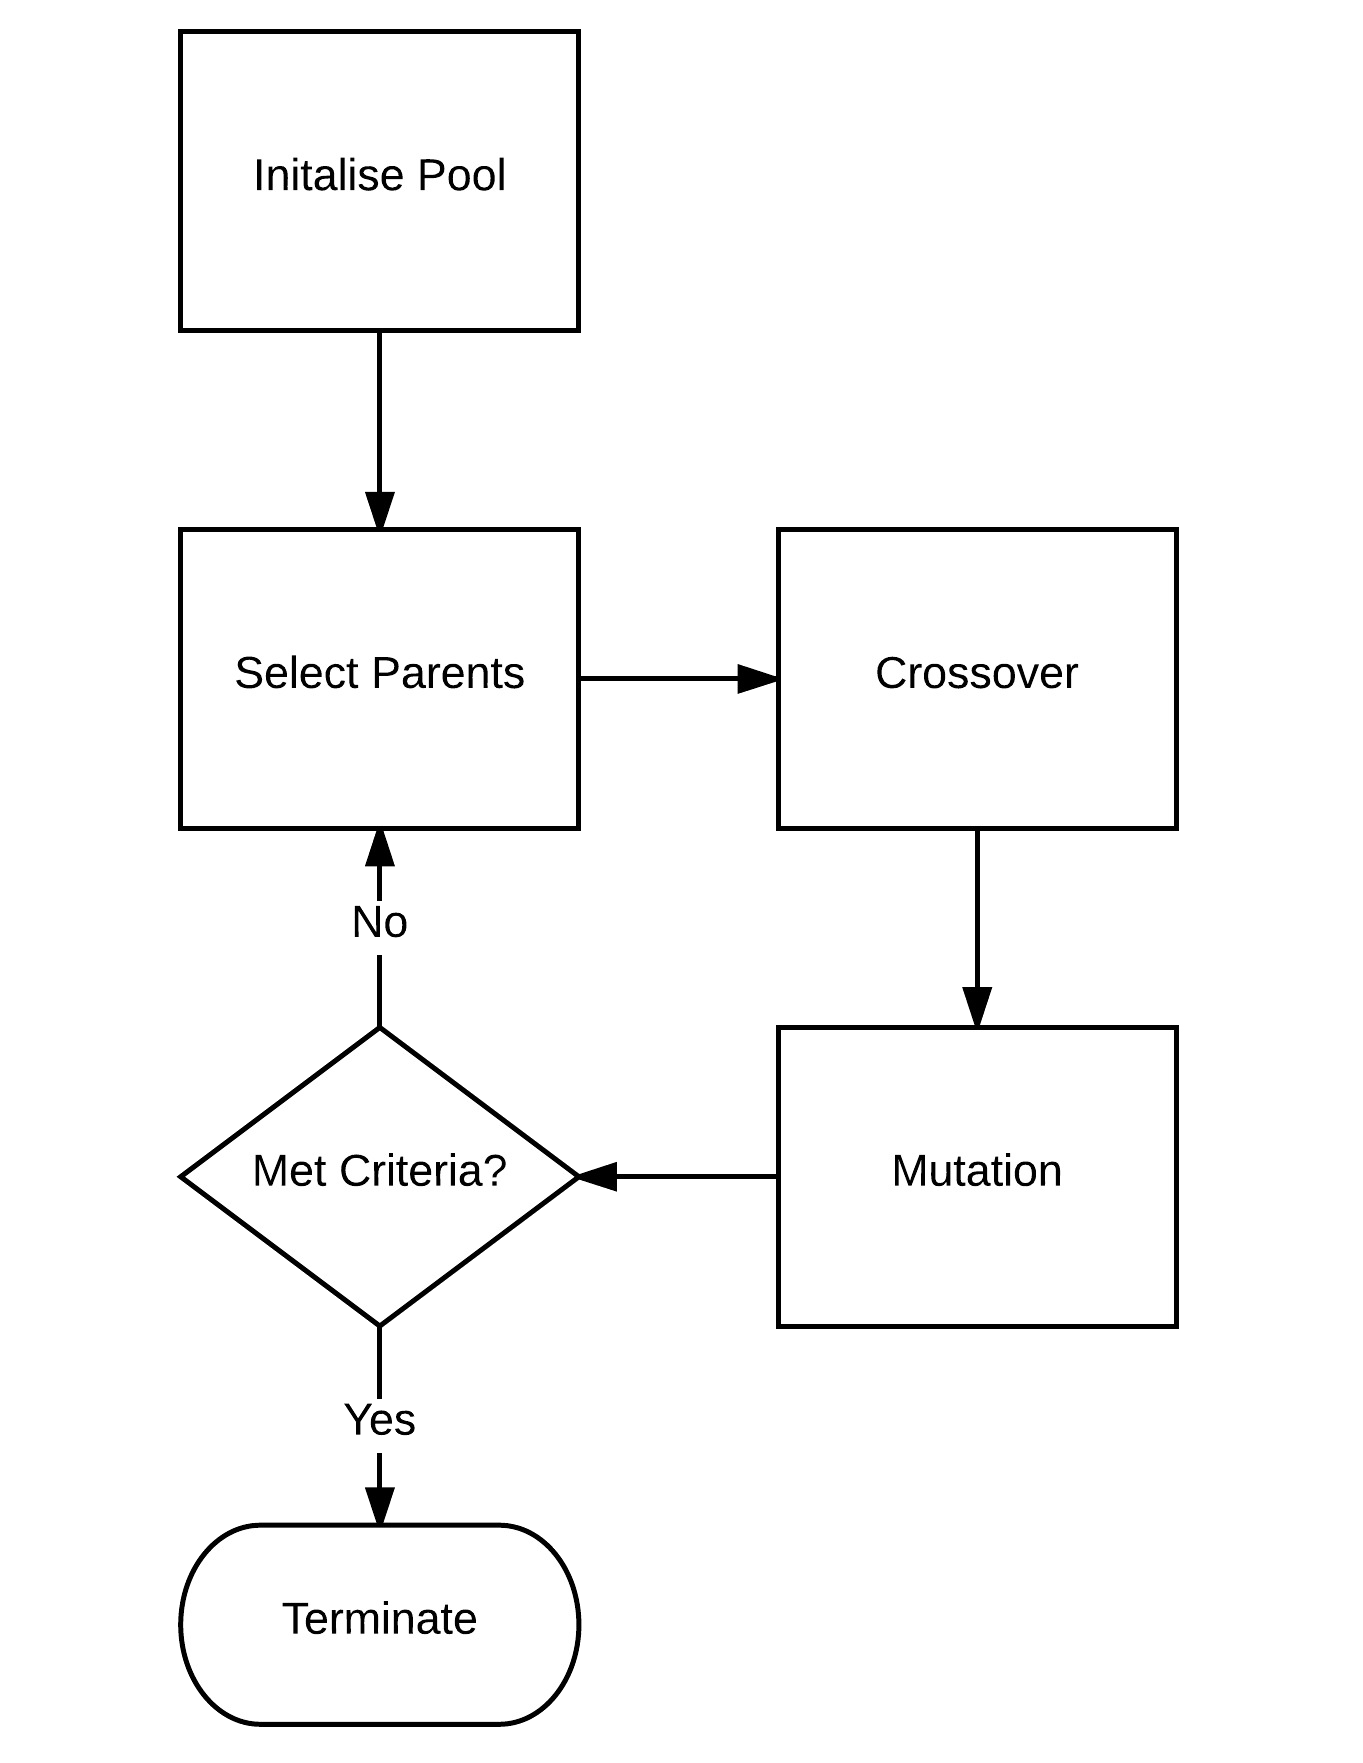
\includegraphics[width=0.5\textwidth]{GA_Structure}
	\caption{The basic structure of a Genetic Algorithm.}
	\label{struct}
\end{figure}
\noindent
A Genetic Algorithm is an algorithm that uses natural selection, or survival of the fittest, to find a solution to a problem. All Genetic Algorithms follow a similar, if not identical structure (figure \ref{struct}). However, the elements of this structure are highly customised for each specific application. Before going into detail about these elements, the concept of chromosomes and fitness must first be introduced.
\par
Chromosomes are one of the most important parts of a GA, their only purpose is to store the potential solutions of the problem. How chromosomes store these solutions is up to the constructor of the GA, commonly however they are a single string that might represent a binary number, or possibly a list of the problem's variables. The components that make up the chromosome are referred to as genes, in a chromosome described as a binary number, each 1 or 0 is a gene. In the research algorithm a chromosome is a tour. Each city in the given Travelling Salesman Problem is a gene, and the order of the genes in the chromosome describes the order that the cities should be visited in. Another thing to note about chromosomes is their fitness. The fitness function of a GA describes how fit a particular chromosome is as a solution. How this fitness works, and how fitnesses are compared is again nearly entirely up to the constructor of the GA.

\subsection{Initialisation of the Pool}
\par
The first step in the execution of a Genetic algorithm is the generation of the pool. The pool is a collection of chromosomes that can be described as the "current generation". This pool is initialised by randomly generating chromosomes until the pool is filled, in the case of the research algorithm, this was done by shuffling the list of cities to construct a tour. Shuffling a list that contains each city only once eliminates the possibility of missing or having duplicate cities within the chromosome which is one of the constraints of the Travelling Salesman Problem. The number of chromosomes in the pool is usually a fixed number, however adaptive pool sizing does exist only fixed pool size was used in this research \cite{populationsize}. 
\subsection{The Main Loop}
\par
This next section comprises the main body of the GA. Every time this loop is completed, a generation has passed. Throughout the next sections, the methods used in the research algorithm will be used as examples.
\subsubsection{Parent Selection}\label{parents}
\par
Parent selection is the first step of each generation. The flow of Figure \ref{struct} suggests that all parents are selected before Crossover, however in reality it is easier and potentially more efficient to do both steps concurrently, thus you select two parents, breed them (Crossover) and repeat until a new pool is constructed.
\par
Parents can be selected in many ways, however usually the fitness of the parents is used in some way to select them. For example, in the research algorithm a method called roulette wheel selection was used (INSERT SOME REFERENCE HERE), in this method all chromosomes in the pool take up an area on a wheel proportional to the fitness of the chromosome. This created some issues within the research algorithm as the fitness function returns the total distance of the chromosome. Thus, the smaller the distance, the better the chromosome. In order to get the correct probability of selection, the fitnesses needed to be 'inverted'. This was done with two equations: 
\[ inv = minFit + maxFit\]
\[ p = (inv - fitness)/totalInvFitness\]
Where $inv$ is the 'Inversion constant', $minFit$ is the smallest/best fitness in the pool, $maxFit$ is the largest/worst fitness in the pool, $p$ is the probability of selection, $fitness$ is the fitness of a chromosome, and $totalInvFitness$ is the sum of all inverted fitnesses in the pool.
\par
Using these equations, the probability of selection for each chromosome in the pool could be calculated, thus allowing for parents to be selected from the pool using these probabilities.
\subsubsection{Crossover}\label{crossover}
\par
\begin{figure}[H]
\textit{Step 1: The children start as duplicates of the parents that have been selected. Also a range of genes is randomly selected, in this example genes 3 to 5 and they are shown in green.}
\[Parent\, 1: [0,3,\colorbox{green}{2,5,1},4]\]
\[Parent\, 2: [1,3,\colorbox{green}{5,0,4},2]\]
\[Child\, 1: [0,3,\colorbox{green}{2,5,1},4]\]
\[Child\, 2: [1,3,\colorbox{green}{5,0,4},2]\]
\textit{Step 2: From the second child, the genes contained in selected range of the first parent are removed. The same thing is done to the first child using the second parent.}
\[Parent\, 1: [0,3,\colorbox{green}{2,5,1},4]\]
\[Parent\, 2: [1,3,\colorbox{green}{5,0,4},2]\]
\[Child\, 1: [-,3,\colorbox{green}{2,-,1},-]\]
\[Child\, 2: [-,3,\colorbox{green}{-,0,4},-]\]
\textit{Step 3: The remaining genes in the children must be moved outside the range selected in step 1, without changing the order the are in.}
\[Parent\, 1: [0,3,\colorbox{green}{2,5,1},4]\]
\[Parent\, 2: [1,3,\colorbox{green}{5,0,4},2]\]
\[Child\, 1: [3,2,\colorbox{green}{-,-,-},1]\]
\[Child\, 2: [3,0,\colorbox{green}{-,-,-},4]\]
\textit{Step 4: Finally the genes selected in the first parent are moved into the now open space in the second child. The same goes for the second parent and first child.}
\[Parent\, 1: [0,3,\colorbox{green}{2,5,1},4]\]
\[Parent\, 2: [1,3,\colorbox{green}{5,0,4},2]\]
\[Child\, 1: [3,2,\colorbox{green}{5,0,4},1]\]
\[Child\, 2: [3,0,\colorbox{green}{2,5,1},4]\]
\caption{Example of the crossover method used in the research algorithm. \label{fig:cross}}
\end{figure}
Crossover (also known as breeding) is when two chromosomes, called parents, are 'crossed' together to produce one or more children. There are many ways of doing this, from slicing the parents in half and swapping the ends, to more complicated methods like the one used in the research algorithm shown in Figure \ref{fig:cross}. 
\subsubsection{Mutation}
\par
\begin{figure}[H]
\[Before: [0,3,\colorbox{green}{2},5,1,\colorbox{red}{4}]\]
\[After: [0,3,\colorbox{red}{4},5,1,\colorbox{green}{2}]\]
\caption{Example of the swap mutation used in the research algorithm. \label{fig:mut}}
\end{figure}
Every child produced in Section \ref{crossover} has a chance of mutation, this is when the chromosome is subjected to a small but random change. In the case of the research algorithm, a specific form of mutation called swap mutation was used where two genes within the chromosome are randomly selected and then swapped, this is shown in Figure \ref{fig:mut}, this particular method of mutation does not invalidate the tour a chromosome describes, since it does not cause duplicate cities nor does it remove cities. Also, in the research algorithm, a chance of mutating multiple times was used, with each subsequent mutation being less and less probable.
\subsection{Termination}
\par
The final step in the Genetic algorithm is termination. At the end of every generation, it is questioned whether the GA has met a specific criterion, if it has then the GA terminates and the best solution in the gene pool is the solution you finish with, otherwise it continues and begins a new generation.
\par
The criteria for termination can be nearly anything and are usually rather specific to the problem, however there are some generic ones, for example having found a solution that is fitter than a given solution or having completed a given number of generations.
\subsection{The Research Framework}
\par
The Genetic Algorithm that was constructed for this research is divided into two components, the first being the Genetic Algorithm Framework, and the second being a script which integrates with the framework \cite{Code}.
The GAFramework is actually quite a simple program, it was designed for the research, however even though the research was specifically on the Traveling Salesman Problem, the GAF is capable of being used for any problem. It simply passes data to the scripts and provides the scripts some generic functionality such as a chromosome object and a loop function.
The script is the main bulk of the program as it is responsible for defining and solving a specific problem. The script constructed to solve the research problems was designed to be a generic script for Traveling Salesman Problems, when provided with a raw text file containing either a distance matrix or the coordinates for each city, it will proceed to solve the problem regardless of size. The script can also be given variables such as the size of chromosome pool, or the percentage of the pool to make elites. 

